\section{Experimental Validation}
\label{Sec:Experiments}

This section discusses or tries to answer several key questions by
simulating the Trinity system described later.
Will Cerberus improve application performance by utilizing burst buffer nodes?
Will job demand on burst buffer effect Cerberus?
Why bother to model the job execution in 3 phases?
Can dynamic programming based optimization help Cerberus further
improve application performance?

\subsection{Simulation Settings}
We consider simulating the full Trinity super computer\cite{TrinitySystem}.
The number of compute nodes on Trinity is about 18936,
e.g. 9436 Intel Haswell nodes
and at least 9500 Intel Xeon Phi nodes.
There are 16 cores on each processor, thus totally 302976 cores.
In the following experiments, we compare two identical system except that
IO nodes are replaced by the same number of burst buffer nodes.
Eventually Trinity plans to delivery up to 576 burst buffer nodes of 3.7 PB,
consisted of Trinity IO nodes with PCIe SSD card.
They are globally accessible as intermediate storage and distributed among cabinets.
Sequential read/write between burst buffer and compute nodes is 8.0 GB/s.
Bandwidth between CPU node and IO node is set to 2.5 GB/s.
Job trace is from ANL's Blue Gene Intrepid system
from January to September 2009\cite{JobTrace}.
We extract two critical fields from this jobs trace: running time and
number of cores user requested.
This trace contains 68936 jobs but
only the first 1185 jobs are considered in this section's simulation.
We patched 3 fields to each job's log entry: the amount of input data $data\_in$,
the amount of written data during checkpointing $data\_run$
and the amount of output data $data\_out$.
We assume they follows uniform distribution with
low boundary 1 TB and high boundary 60 TB.
The patches 3 fields may or may not be used in scheduling,
depends on both the model of the jobs and the experiment scenario.


\subsection{Cerberus vs. 1-Phase Batch Scheduler}
\label{Sec:Sim:DirectIOvsBB}
In this section, we demonstrate that by utilizing burst buffer nodes,
job scheduler could improve the applications' performance.
Figure~\ref{Fig:DirectIOvsBBResponse} compares CDF of the response time of 1000 jobs.
When scheduler can allocate burst buffer to jobs (denoted as Plain BB),
all jobs finish in 360,000 seconds counting from their submission time.
However, the worst case in system without burst buffer (denoted as Direct IO) is catastrophical.
There are jobs that takes almost 1,400,000 seconds to finish,
almost as 4 times slow as the most non-responsive job in system equipped with burst buffer.
In average case, more than 90\% of the jobs scheduled by Cerberus response faster than 1-Phase Batch scheduler.
The improvement mainly comes from the difference of IO operation efficiency between
traditional IO nodes and burst buffer nodes.
There are only less than 10\% of the jobs response quicker without needing burst buffer.

Using the collected completion time, we can calculate system's throughput over time sequence.
Figure~\ref{Fig:DirectIOvsBBThroughput} shows the number of tasks finished
in a fixed time unit (500 seconds) for system using burst buffer nodes and not.
It takes more than 1,382,769 seconds for the system without burst buffer nodes to
server all 1000 jobs.
The last job is job \#1150, which requested 4096 cores and 49 TB data space.
It starts at 1169 seconds and finishes at 1,383,938 seconds.
In contrast, when system installed burst buffer nodes,
it accomplishes the same 1185 jobs in 336,396 seconds.
Job \#1150 is the second last job finished, but both its completion time and response time
are significantly reduced, 268701 and 267531 seconds respectively.
As indicated by the horizontal lines (green for Direct IO and yellow for Plain BB),
the ratio of average throughput between two systems is about 4, namely 1.769 to 0.431.
This approximately coincides with the 4-time response speedup,
made possible due to burst buffer equipments.


\begin{figure}[!t]
        \centering
        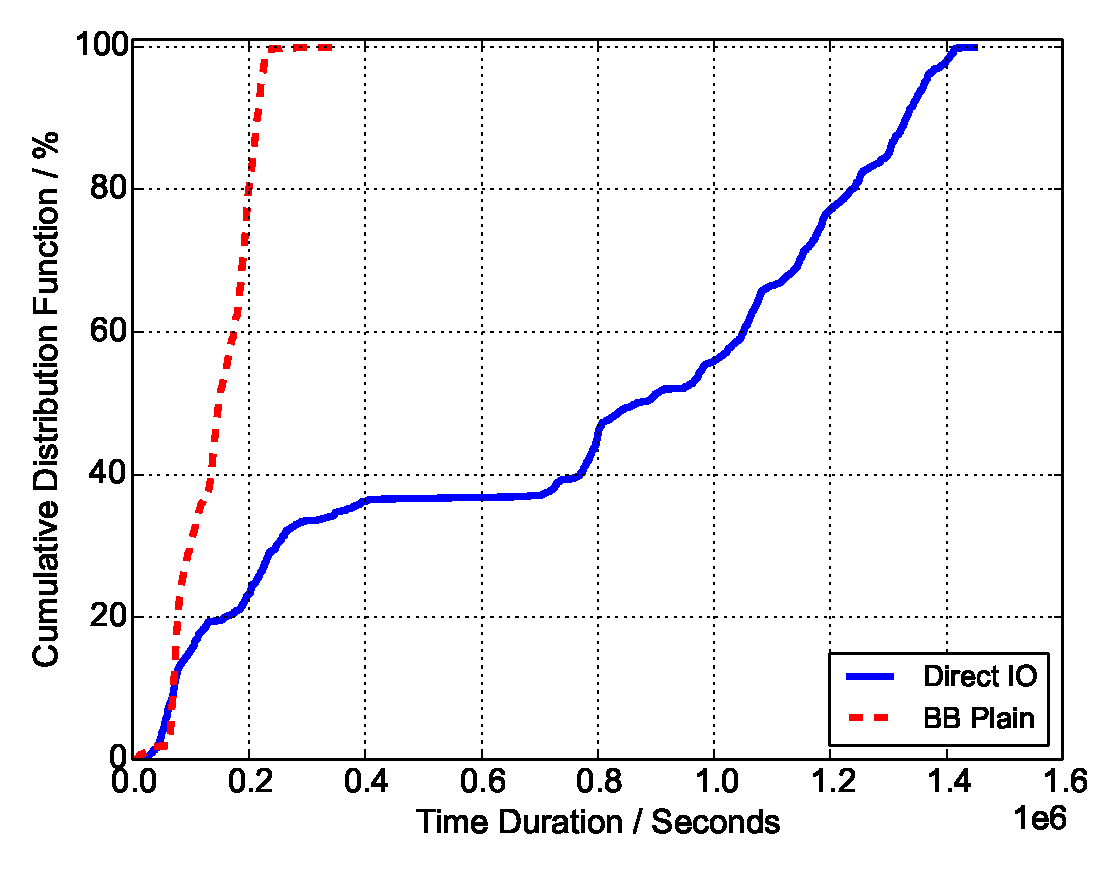
\includegraphics[width=3.2in]{DrawDirectIOvsBB/1000jobs_direct_vs_bb_response}
        \caption{Job Response Time, IO Node Only vs. Burst Buffer System}
        \label{Fig:DirectIOvsBBResponse}
\end{figure}

\begin{figure}[!t]
        \centering
        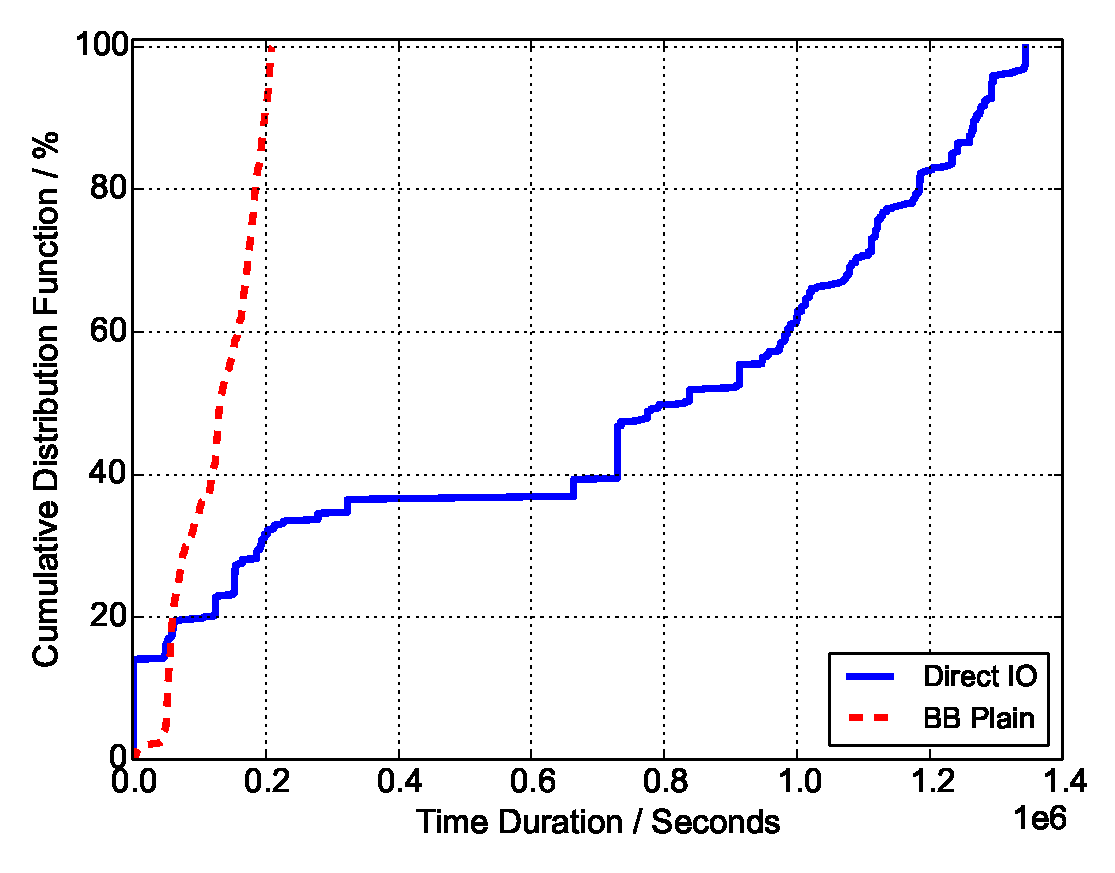
\includegraphics[width=3.2in]{DrawDirectIOvsBB/1000jobs_direct_vs_bb_wait}
        \caption{Job Wait Time, IO Node Only vs. Burst Buffer System}
        \label{Fig:DirectIOvsBBWait}
\end{figure}

\begin{figure}[!t]
        \centering
        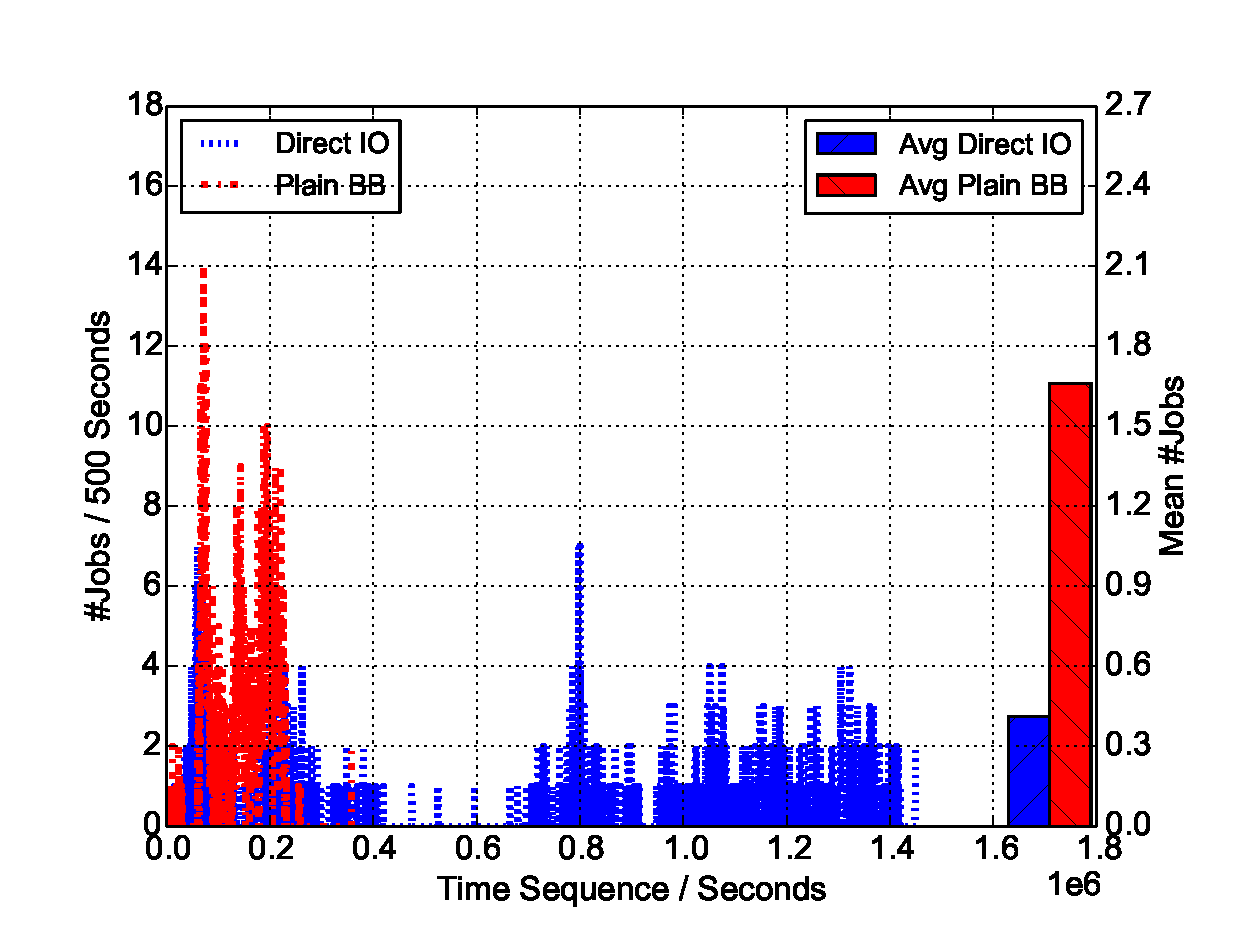
\includegraphics[width=3.2in]{DrawDirectIOvsBB/1000jobs_direct_vs_bb_throughput}
        \caption{System Throughput, IO Node Only vs. Burst Buffer System}
        \label{Fig:DirectIOvsBBThroughput}
\end{figure}


\subsection{Cerberus vs. Demand Granularity}
In this section we validate our 3-phase model.
Applications are benefited when scheduler dividing jobs into 3 separated phases and 
scheduling are based on corresponding burst buffer demand in each phase.
This suggests that user should provide burst buffer demand as granular as possible.

In Figure~\ref{Fig:3Pvs1PResponse}, we plot 3 different scheduling results by 3 FCFS scheduler.
Jobs in the first case, denoted as Direct BB, are modeled as just 1 phase because user just provides
a general burst buffer demand throughout entire application life time.
We assume this demand is the $\max \{data\_in, data\_out, data\_run\}$.
This is the traditional scheduling scheme except job has additional
burst buffer demand and scheduler must subject to burst buffer capacity constraint.
Jobs in the second and third cases have 3 phases and are scheduled by Cerberus.
However, in the second case, denoted as Plain BB 1D, Cerberus only knows the overall burst buffer demand,
same as the information in case 1.
In the 3rd case, named Plain BB 3P, users kindly provided all the burst buffer demand in all 3 phases.
This is the same case as in section~\ref{Sec:Sim:DirectIOvsBB} when we demonstrating burst buffer is beneficial.
We simulate the 3 cases with the same generated random data volume.
For 1-phase-modeled jobs, scheduler will make decision based on $\max \{data\_in, data\_out, data\_run\}$
since we assume user will only tell the upper bound of its application's demand.
However, in simulation, we use the generated data amount as the same as 3-modeled jobs.
%Response time of system without burst buffer devices are also plotted for comparison.

Unsurprisingly, jobs' response time is improving as long as they could utilizing burst buffer.
Let's compare scheduling results of 1-phase and 3-phase, both of which only have rough data information of application.
More than 60\% of the 3-phase-modeled jobs finish faster than 1-phase-modeled jobs.
The longest 3-phase-modeled job takes 400,000 seconds to finish while the slowest 1-phase-modeled job
needs about 540,000 seconds to finish.
The improvement is about 26\% for the worst case.
The reason of such improvement is as follows.
For the 1-phase-modeled jobs, burst buffer nodes will be exclusively taken by scheduled jobs
throughout their lifetime.
In contrast, each time a 3-phase-modeled job finish inputing, running or outputing,
Cerberus will reclaim burst buffer and CPU resources.
This gives Cerberus more opportunity to schedule the system resources.
At last, when comparing the case of 3-phase IRO with 3-phase D, we find another advantage of our 3-phase model.
If benign users can provide finer-grain information of data/IO demand,
Cerberus can programme each queue separately and get better scheduling result.
In our simulation, when Cerberus knows more about application's demand in different phases,
the worst absolute response time is less than 300,000 seconds.
This is 25\% improvement to 3-phase-modeled jobs when Cerberus only knows the upper bound of data demand,
44\% better than the slowest 1-phase-modeled job.
In average case, 80\% of the 3-phase-modeled jobs scheduled by Cerberus finish earlier than 1-phase-modeled jobs,
on the same condition that the same amount of burst buffer nodes are available to applications.
Meanwhile, more than 90\% of the jobs takes less time if user specifies data usage demand
at each phase to Cerberus.

Figure~\ref{Fig:3Pvs1PThroughput} describes system throughput of these three different scenarios.
It helps us examine the performance of the scheduling in time sequence.
For 1-phase-modeled job, we can see an obvious `throughput gap'
from 150,000 second to 250,000 second approximately.
This is the result of too aggressive scheduling at the beginning.
For the case of 3-phase D, throughput also starts provocatively,
but not as provocatively as 1-phase scheduling case;
it is then calmed due to frequent resource release,
indicated by multiple crests and troughs from 0 to 350,000 seconds.
The 3-phase IRO runs counter to the both previous cases.
Even though beginning with throughput trough,
Cerberus manages to make the system having high throughput from 50,000 to 250,000 seconds,
during which system can achieve throughput around 10 to 12 per 500 seconds. 
In average, the throughput of 3-phase IRO case is 1.670 jobs / 500 seconds.
It is 51.82\% higher than the Direct BB case (1.101 jobs / 500 seconds) and
17.69\% higher than the Plain BB 1D case (1.419 jobs / 500 seconds).
We believe this validates the indispensable 3 phase job model and
the necessity that user provides data capacity demand for each phase.


\begin{figure}[!t]
        \centering
        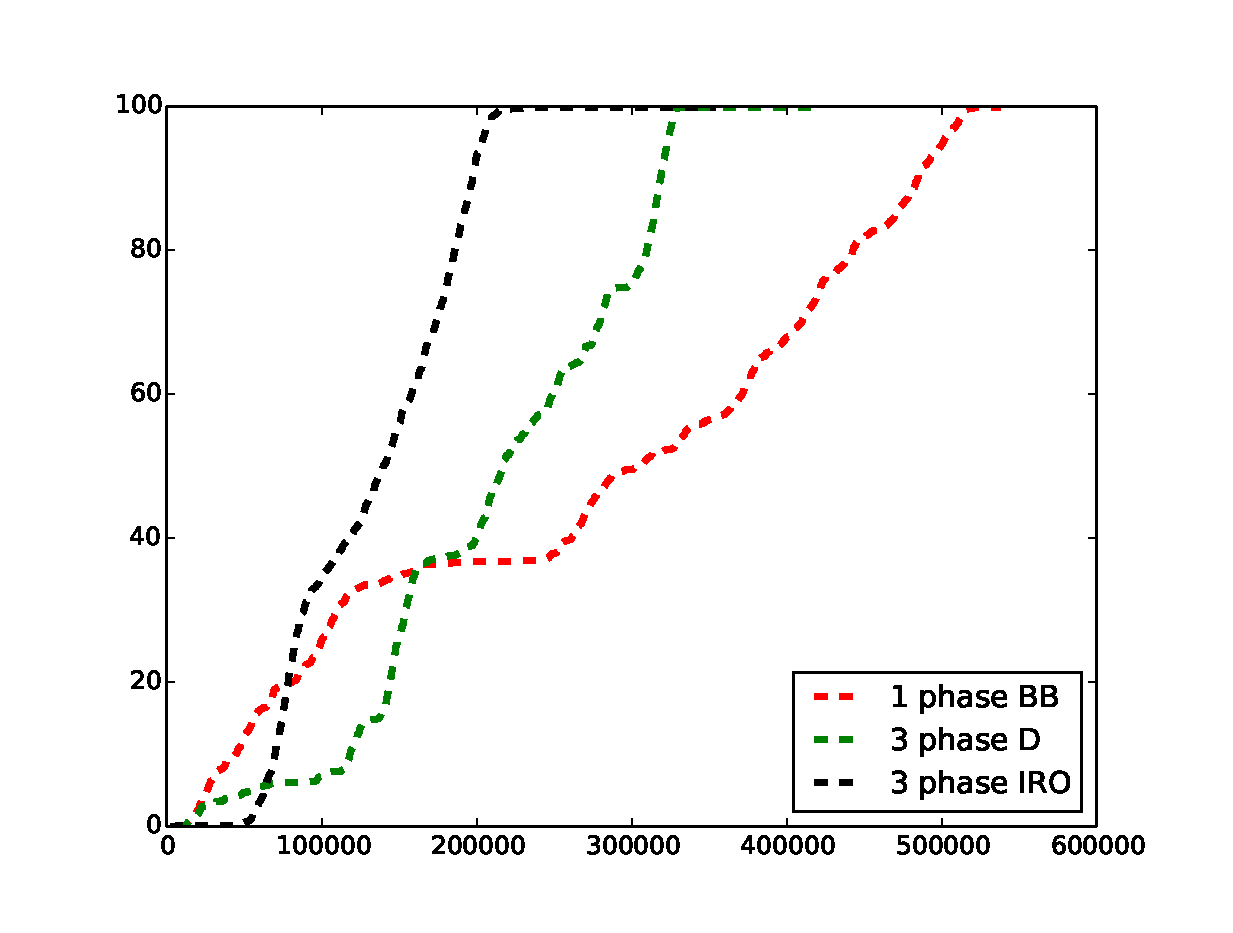
\includegraphics[width=3.2in]{Draw3Pvs1P/1000jobs_3p_vs_1p_response}
        \caption{Job Response Time, 1 Phase Model vs. 3 Phase Model}
        \label{Fig:3Pvs1PResponse}
\end{figure}

\begin{figure}[!t]
        \centering
        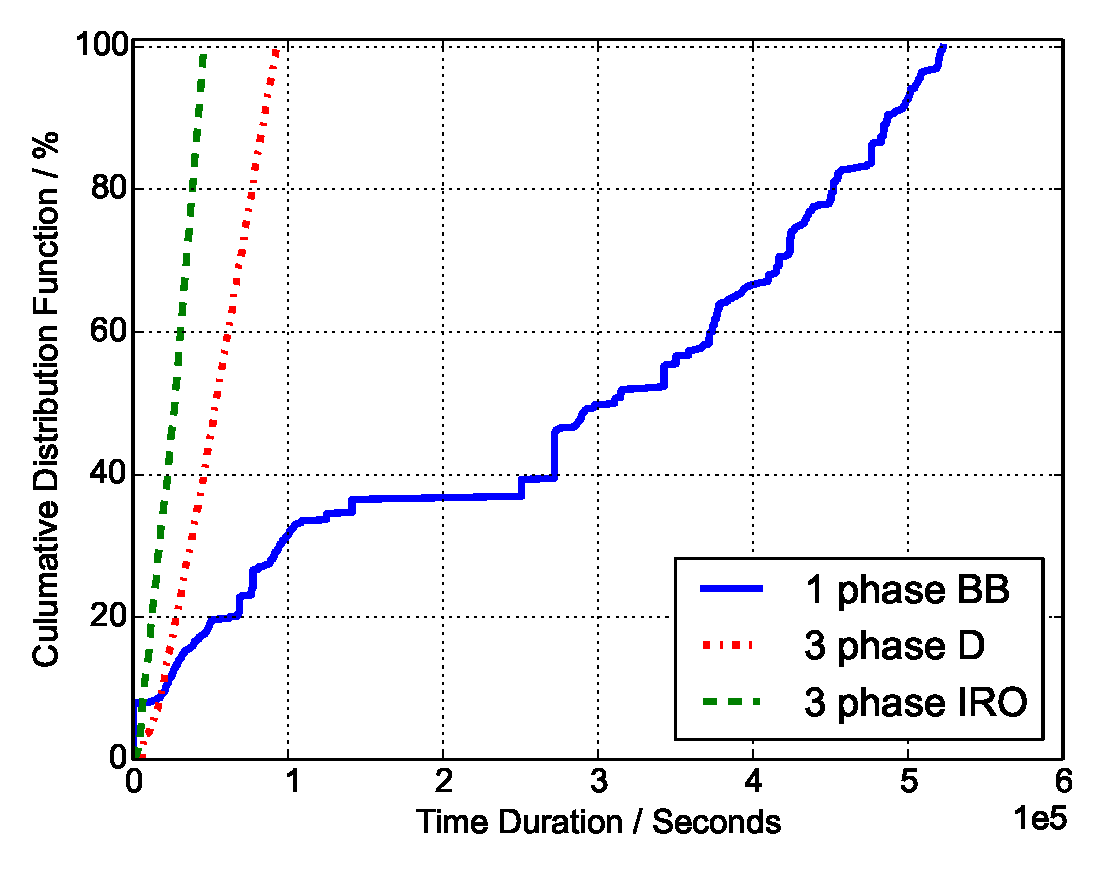
\includegraphics[width=3.2in]{Draw3Pvs1P/1000jobs_3p_vs_1p_wait_in}
        \caption{Job Wait Input Time, 1 Phase Model vs. 3 Phase Model}
        \label{Fig:3Pvs1PWaitIn}
\end{figure}
\begin{figure}[!t]
        \centering
        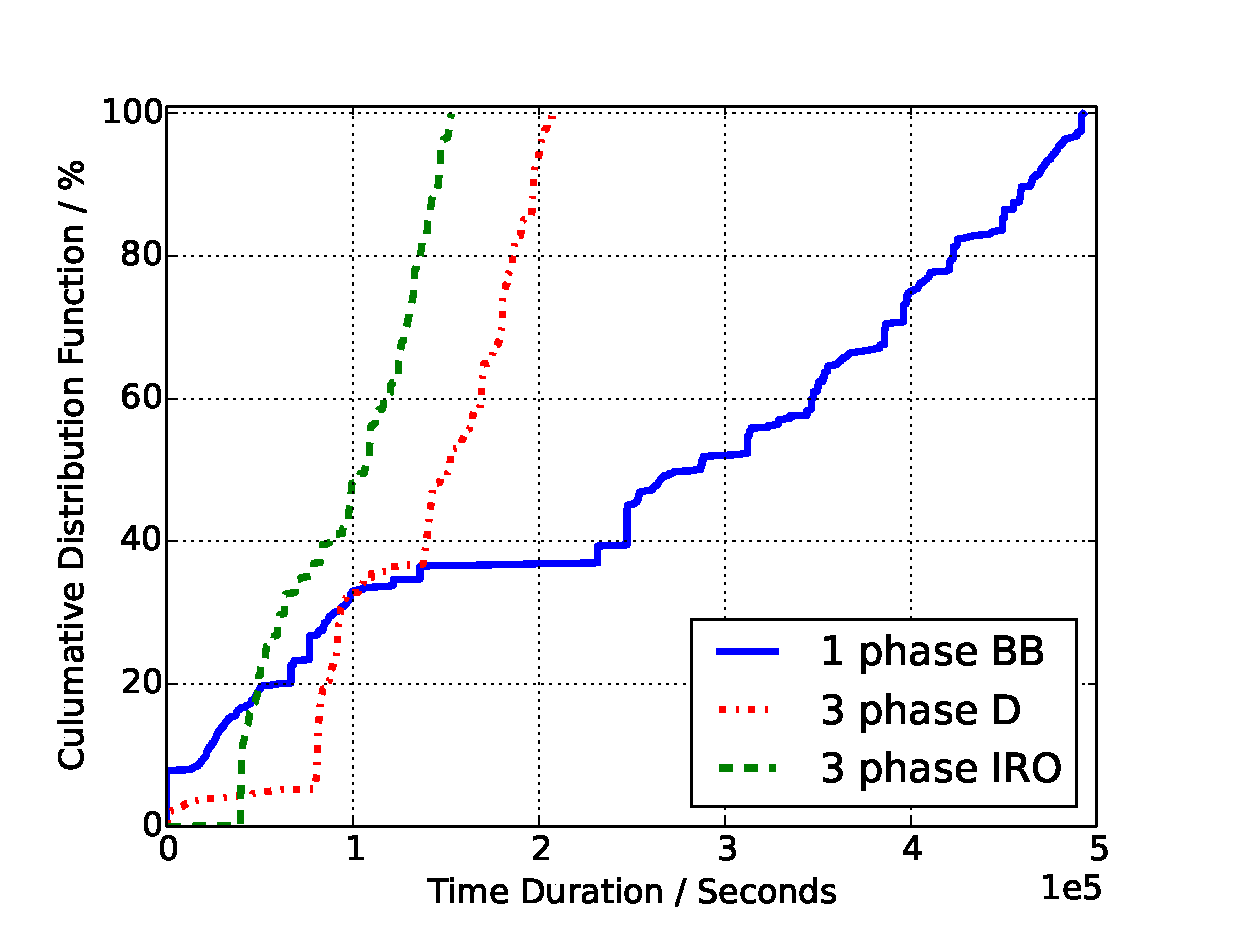
\includegraphics[width=3.2in]{Draw3Pvs1P/1000jobs_3p_vs_1p_wait_run}
        \caption{Job Wait Run Time, 1 Phase Model vs. 3 Phase Model}
        \label{Fig:3Pvs1PWaitRun}
\end{figure}
\begin{figure}[!t]
        \centering
        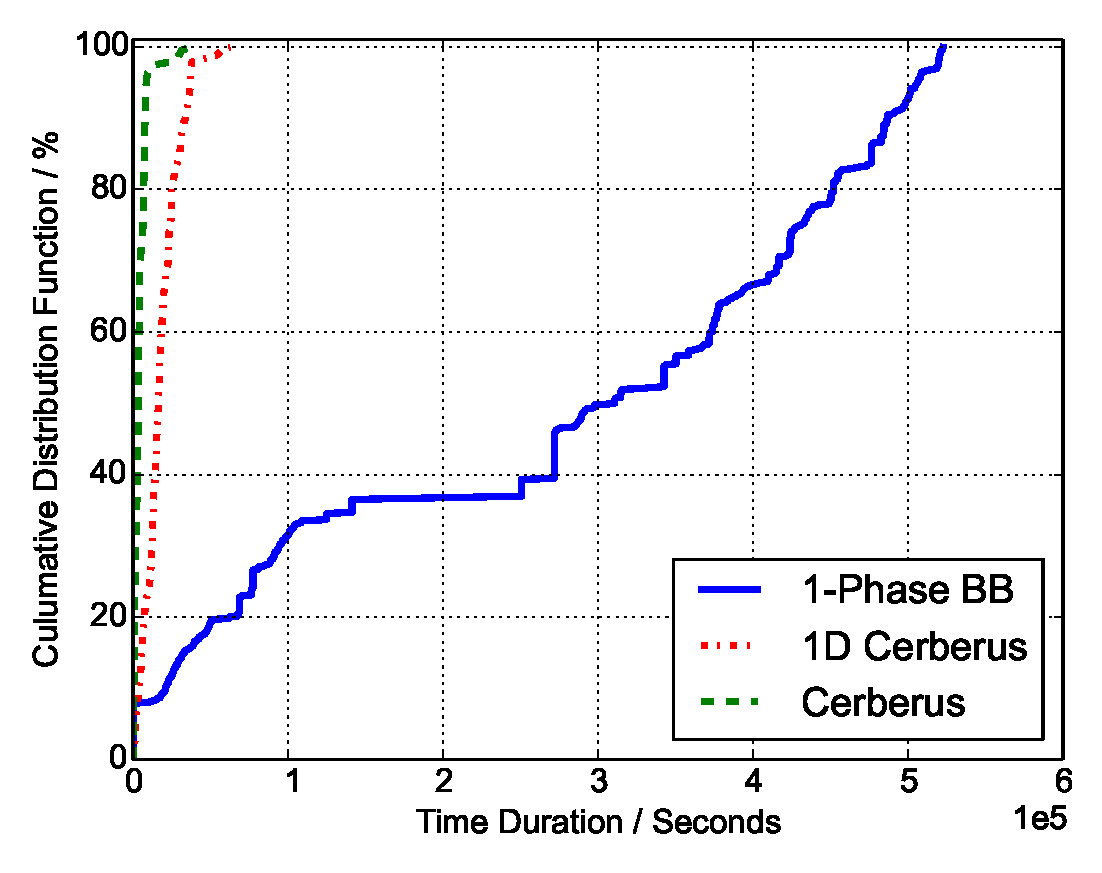
\includegraphics[width=3.2in]{Draw3Pvs1P/1000jobs_3p_vs_1p_wait_out}
        \caption{Job Wait Output Time, 1 Phase Model vs. 3 Phase Model}
        \label{Fig:3Pvs1PWaitOut}
\end{figure}

\begin{figure}[!t]
        \centering
        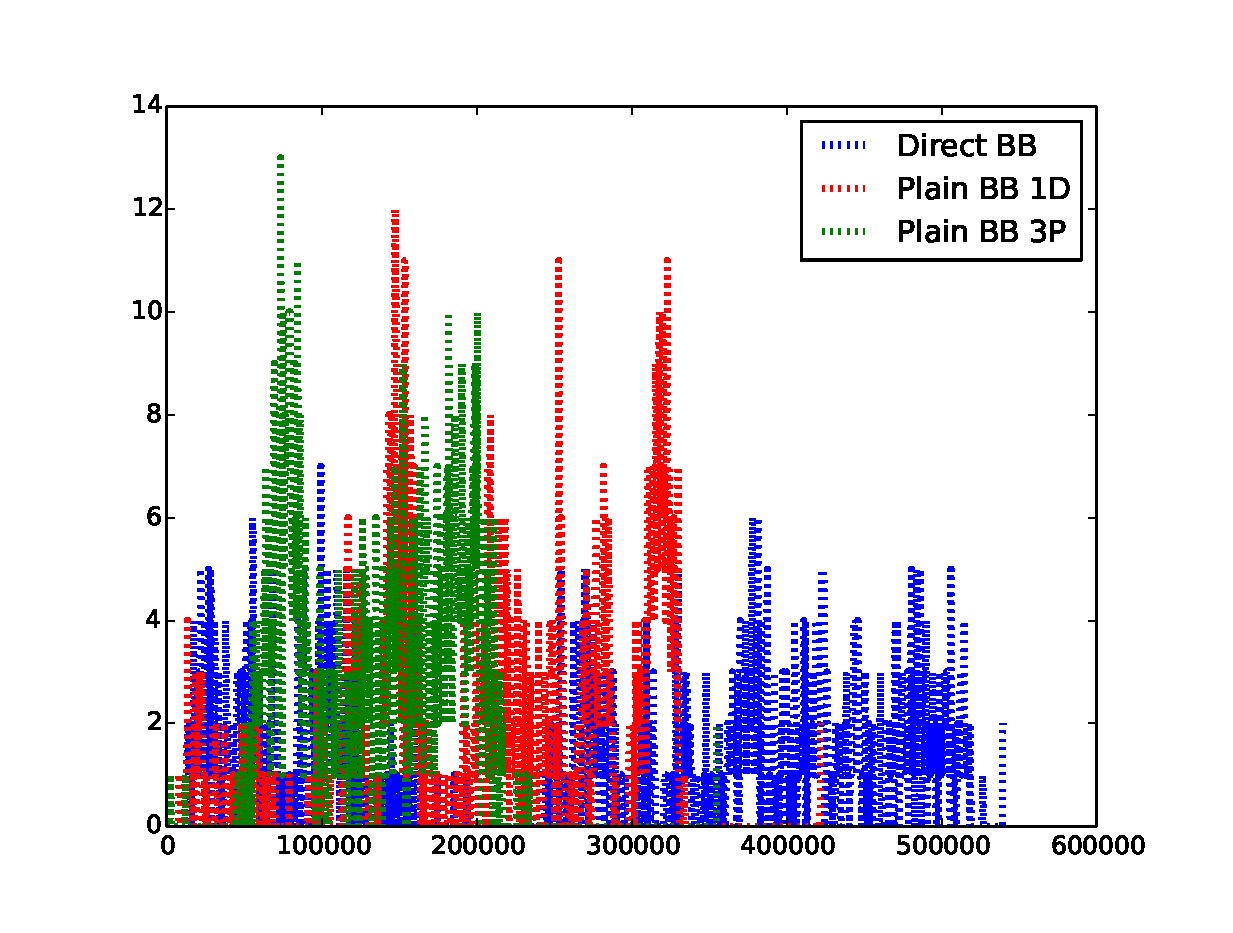
\includegraphics[width=3.2in]{Draw3Pvs1P/1000jobs_3p_vs_1p_throughput}
        \caption{System Throughput, 1 Phase Model vs. 3 Phase Model}
        \label{Fig:3Pvs1PThroughput}
\end{figure}



\subsection{Cerberus vs. Cerberus with Optimization}
If we consider optimizing either burst buffer's data throughput or the parallelism across jobs,
dynamic programming based job scheduler can further reduce jobs' wait time.
We plot in Figure~\ref{Fig:DPvsFIFOResponse} the resulting response time of
three version of Cerberus scheduler differs in
how they handle jobs in their queues (input queue, run queue, and output queue).
The first scheduler uses naive first come first serve (FCFS) policy.
Whoever at the front of queue are considered favorably.
The second and third version treat jobs in run queue identically.
They choose jobs according to the optimization solution given by Equation~\ref{Equ:MaxProductRecursion}
However, they treat jobs in the input queue and output queue differently.
The second version will select these jobs in its queue so that
volume of to be transferred data is maximized.
The dynamic programming recursion is Equation~\ref{Equ:MaxTransferDataRecursion}
The third version of Cerberus tries to optimize the number of jobs,
subjecting to burst buffer volume constraint by Equation~\ref{Equ:MaxTaskNumberRecursion}.

As indicated by Figure~\ref{Fig:DPvsFIFOResponse}, response time of
jobs scheduled by both Cerberus version 2 and 3 are reduced.
The most non-responsive job for both Cerberus V2 and V3 is job \#944,
taking 89809 and 88739 seconds respectively.
In contrast, job \#1150 takes 120466 seconds to finish when Cerberus using FCFS.
This is 25.4\% slower than Cerberus V2 and 26.3\% slower than Cerberus V3.
When we consider the overall response time of entire job set,
we see more than 95\% of the tasks response faster when we choose jobs according to
optimization result.
The scheduling results of Cerberus V2 and V3 are fairly closed to each other.
In this simulation, 75\% of the jobs could get better response time
if we maximizing number of parallelable tasks,
versus maximizing transferred data.

We can see in Figure~\ref{Fig:DPvsFIFOThroughput} the throughput of system
when scheduled by 3 different versions of Cerberus.
For optimal Cerberus, job \#944 decides the finishing time of all 1185 jobs.
That is 99244 seconds for Cerberus when it maximizing data throughput
and 93115 seconds for Cerberus when it maximizing parallelable tasks.
The plain Cerberus, scheduling jobs in queue with FCFS policy,
makes system ends its last job, job \#1150, at 132010 seconds.
The worst case completion improvement to FCFS-style Cerberus is
24.8\% for max-BB-style Cerberus and 29.5\% for max-number-task-style Cerberus.
When we look at the time sequence of throughput,
we found the peak value 36 jobs / 500 seconds obtained Cerberus
when maximizing the number of parallel tasks being able to run.
The alternative optimization method, maximizing burst buffer's usage,
could achieve 28 jobs / 500 seconds before 20000 seconds.
The peak throughput of FCFS policy is 22 jobs / 500 seconds around 50000 seconds.
Mean throughputs of these 3 scheduling methods are drawn
as bar chart in Figure~\ref{Fig:DPvsFIFOThroughput}.
Comparing with FCFS Cerberus, max-BB version achieves
34.2\% higher average throughput (6.030 jobs / 500 seconds)
while max-number-task version gives 40.8\% improvement (6.330 jobs / 500 seconds),
that is, extra 6.6\% enhancement to max-BB version.


\begin{figure}[!t]
        \centering
        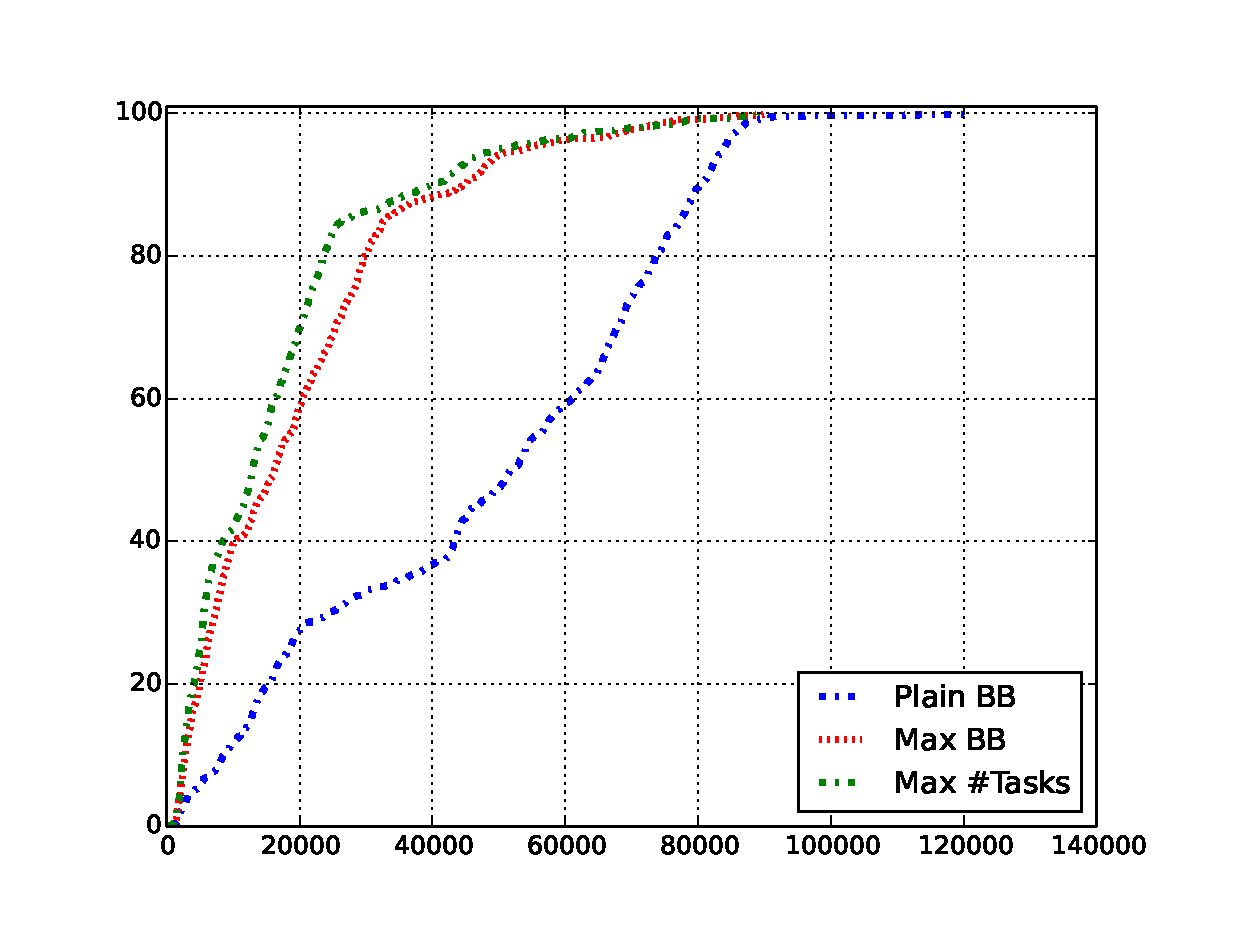
\includegraphics[width=3.2in]{DrawDPvsFIFO/1000jobs_dp_vs_fifo_response}
        \caption{Job Response Time, Dynamic Programming vs. FCFS}
        \label{Fig:DPvsFIFOResponse}
\end{figure}

\begin{figure}[!t]
        \centering
        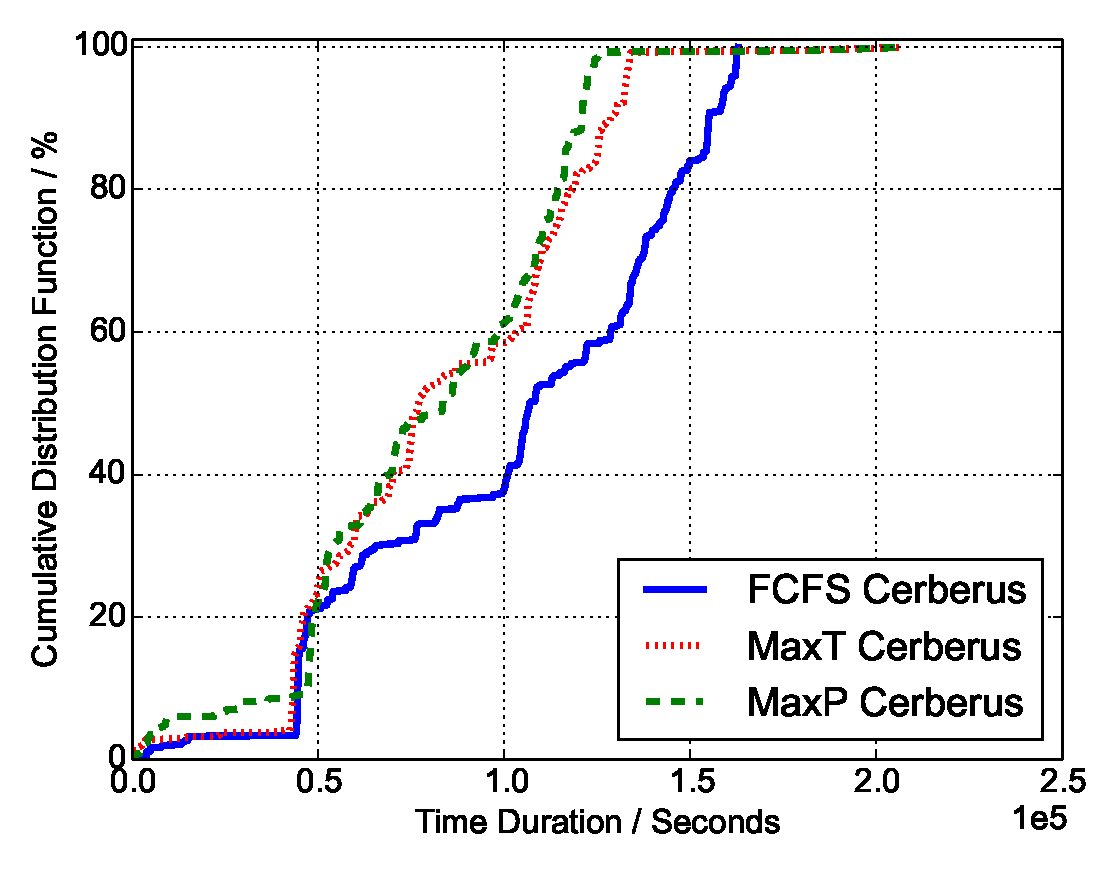
\includegraphics[width=3.2in]{DrawDPvsFIFO/1000jobs_dp_vs_fifo_wait_run}
        \caption{Job Wait Run Time, Dynamic Programming vs. FCFS}
        \label{Fig:DPvsFIFOWaitRun}
\end{figure}

\begin{figure}[!t]
        \centering
        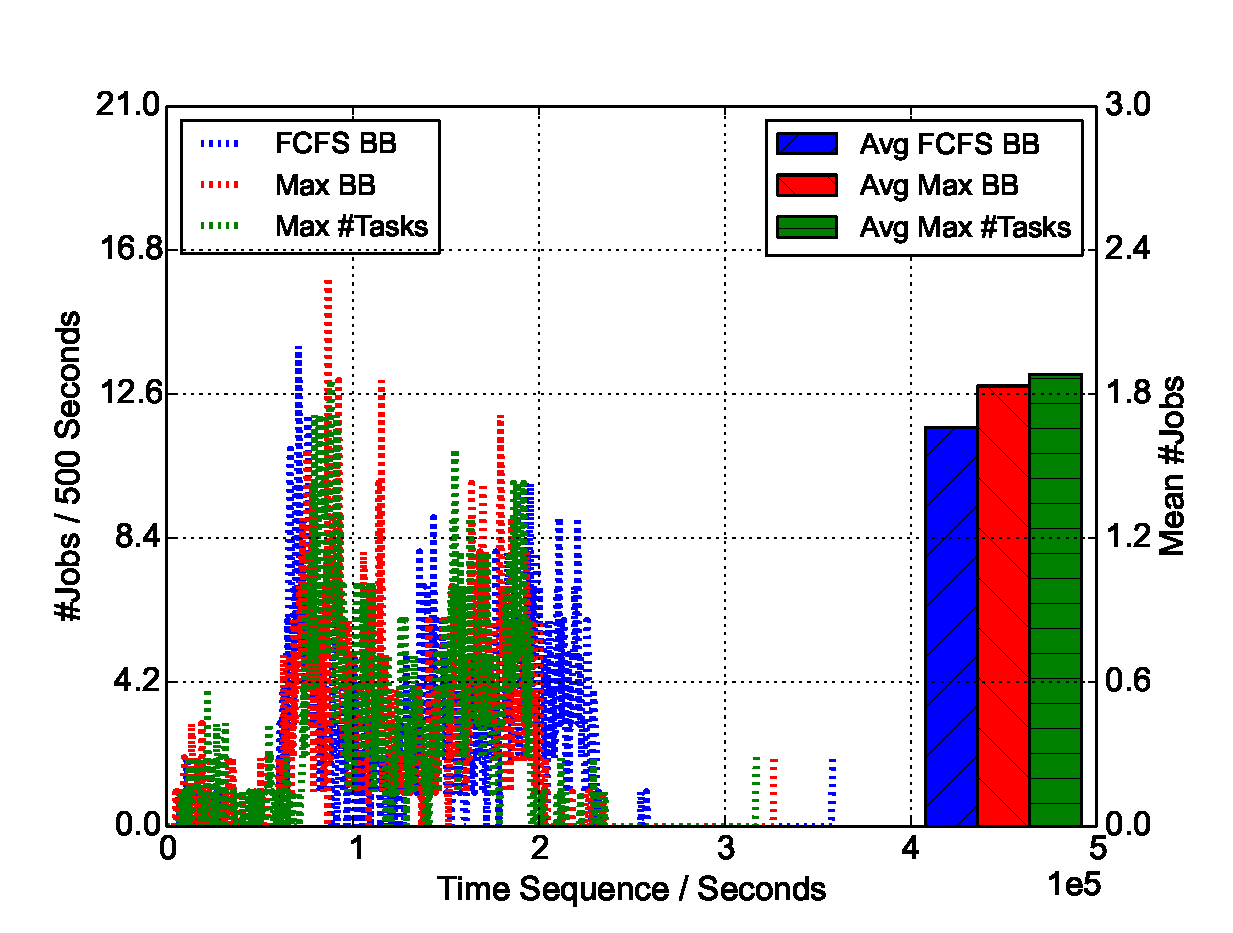
\includegraphics[width=3.2in]{DrawDPvsFIFO/1000jobs_dp_vs_fifo_throughput}
        \caption{System Throughput, Dynamic Programming vs. FCFS}
        \label{Fig:DPvsFIFOThroughput}
\end{figure}




